\documentclass[12pt, a4paper]{article}

% Pakiety podstawowe
\usepackage{polski}
\usepackage[utf8]{inputenc}
\usepackage[margin=2.5cm]{geometry}
\usepackage{tabularx}
\usepackage{graphicx}

\begin{document}

\begin{table}[h!]
\centering
\renewcommand{\arraystretch}{2.5}
\begin{tabularx}{\textwidth}{|p{3cm}|X|p{4.5cm}|}
\hline
\textit{Grupa 6} & \textit{28.10.2026} & \textit{} \\ \hline
\multicolumn{3}{|l|}{\textit{8. Routing}} \\ \hline
\multicolumn{2}{|l|}{\textit{Filip Będkowski, Danylo Drygo}} & \textit{} \\ \hline
\end{tabularx}
\end{table}


\section{Wstęp teoretyczny}

W ramach laboratorium zapoznaliśmy się z zagadnieniem trasowania pakietyzowanych danych w sieciach komputerowych. Trasowanie stanowi kluczowy mechanizm warstwy sieciowej, umożliwiający efektywną wymianę pakietów pomiędzy wyodrębnionymi podsieciami fizycznymi oraz logicznymi.

\subsection{Podstawowe pojęcie}
\begin{itemize}
    \item \textbf{Routing:} trasowanie, „algorytm wyznaczania trasy i wysłanie nią pakietu”
\end{itemize}

\subsection{Istota działania i klasyfikacja routerów}
Router to urządzenie sieciowe, którego podstawowym zadaniem jest analiza adresu docelowego w nagłówku pakietu i podjęcie decyzji o wyborze optymalnego interfejsu wyjściowego. W zależności od skali sieci i wymagań wydajnościowych wyróżnia się:
\begin{itemize}
    \item \textbf{Routery programowe:} zwykłe komputery lub serwery z odpowiednio skonfigurowanym systemem operacyjnym, np. Linux/Unix.
    \item \textbf{Routery klasy Desktop/SOHO:} małe urządzenia integrujące funkcje trasownika, switcha oraz bezprzewodowego punktu dostępowego, powszechne w sieciach domowych.
    \item \textbf{Routery brzegiowe i szkieletowe (EDGE/WAN):} zaawansowane jednostki dedykowane, zdolne do przetwarzania miliardów pakietów na sekundę oraz realizacji zaawansowanej filtracji i funkcji bezpieczeństwa.
\end{itemize}

\subsection{Klasyfikacja algorytmów routingu}
Algorytmy trasowania można klasyfikować według różnorodnych kryteriów funkcjonalnych:
\begin{enumerate}
    \item \textbf{Statyczne vs Dynamiczne:}
    \begin{itemize}
        \item \textit{Statyczne:} trasy wprowadzane są ręcznie przez administratora. Awaria łącza powoduje utratę łączności do czasu ręcznej rekonfiguracji.
        \item \textit{Dynamiczne:} algorytmy na bieżąco analizują topologię sieci w czasie rzeczywistym i automatycznie modyfikują tablice routingu w przypadku wykrycia zmian w stanie łączy.
    \end{itemize}
    \item \textbf{Single-path vs Multi-path:}
    \begin{itemize}
        \item \textit{Single-path:} wyznacza wyłącznie jedną, ścisłą trasę do stacji docelowej.
        \item \textit{Multi-path:} pozwala na równoległe przesyłanie pakietów wieloma alternatywnymi ścieżkami, co podnosi odporność na awarie i zwiększa szybkość.
    \end{itemize}
    \item \textbf{Algorytmy Intradomain vs Interdomain:}
    \begin{itemize}
        \item \textit{Intradomain:} operują wewnątrz jednej domeny. Trasy są zazwyczaj gorsze niż w algorytmie Interdomain. 
        \item \textit{Interdomain:} zarządzają ruchem z uwzględnieniem powiązań między wieloma domenami, dzięki czemu uwzględniają pełną strukturę sieci
    \end{itemize}
    \item \textbf{Algorytmy Link State vs Distance Vector:}
    \begin{itemize}
        \item \textit{Link State:} routery rozsyłają informacje o stanie swoich bezpośrednich łączy do wszystkich węzłów w obszarze. Charakteryzują się szybką zbieżnością, lecz wymagają większej mocy obliczeniowej.
        \item \textit{Distance Vector:} routery cyklicznie przesyłają całą swoją tablicę routingu wyłącznie do bezpośrednich sąsiadów. Metoda prostsza w implementacji, lecz wolniej reagująca na awarie.
    \end{itemize}
\end{enumerate}

\subsection{Routing w architekturze modelu OSI}
Model OSI definiuje hierarchiczną strukturę trasowania opartą na dwóch klasach węzłów oraz trzech poziomach komunikacji:
\begin{itemize}
    \item \textbf{ES (End System):} system końcowy (host), niebiorący udziału w trasowaniu pakietów innych węzłów.
    \item \textbf{IS (Intermediate System):} system pośredniczący (router), realizujący funkcje przekazywania pakietów.
\end{itemize}

Komunikacja i trasowanie odbywają się na następujących poziomach:
\begin{itemize}
    \item \textbf{Poziom 1 (Level 1):} routing ograniczony do jednego obszaru (\textit{area}).
    \item \textbf{Poziom 2 (Level 2):} routing pomiędzy obszarami w granicach tej samej domeny.
    \item \textbf{Routing międzydomenowy: (prawdopodobnie level 3 lub level 1-2)} wykraczający poza obszar pojedynczej domeny routingu.
\end{itemize}
Proces rozpoczyna się od identyfikacji najbliższego systemu IS przez hosty ES. Pakiet adresowany do innego obszaru przekazywany jest przez router Poziomu 1 do najbliższego routera Poziomu 2, a stamtąd trafia bezpośrednio do obszaru docelowego.

\begin{figure}[htbp]
    \centering
    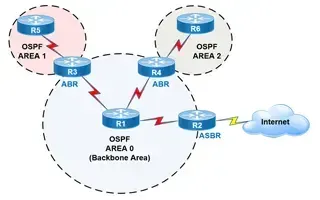
\includegraphics[width=0.63\textwidth]{routing_schematic.png}
    \caption{Schemat poziomów komunikacji i routowania}
    \label{fig:schemat_routowania}
    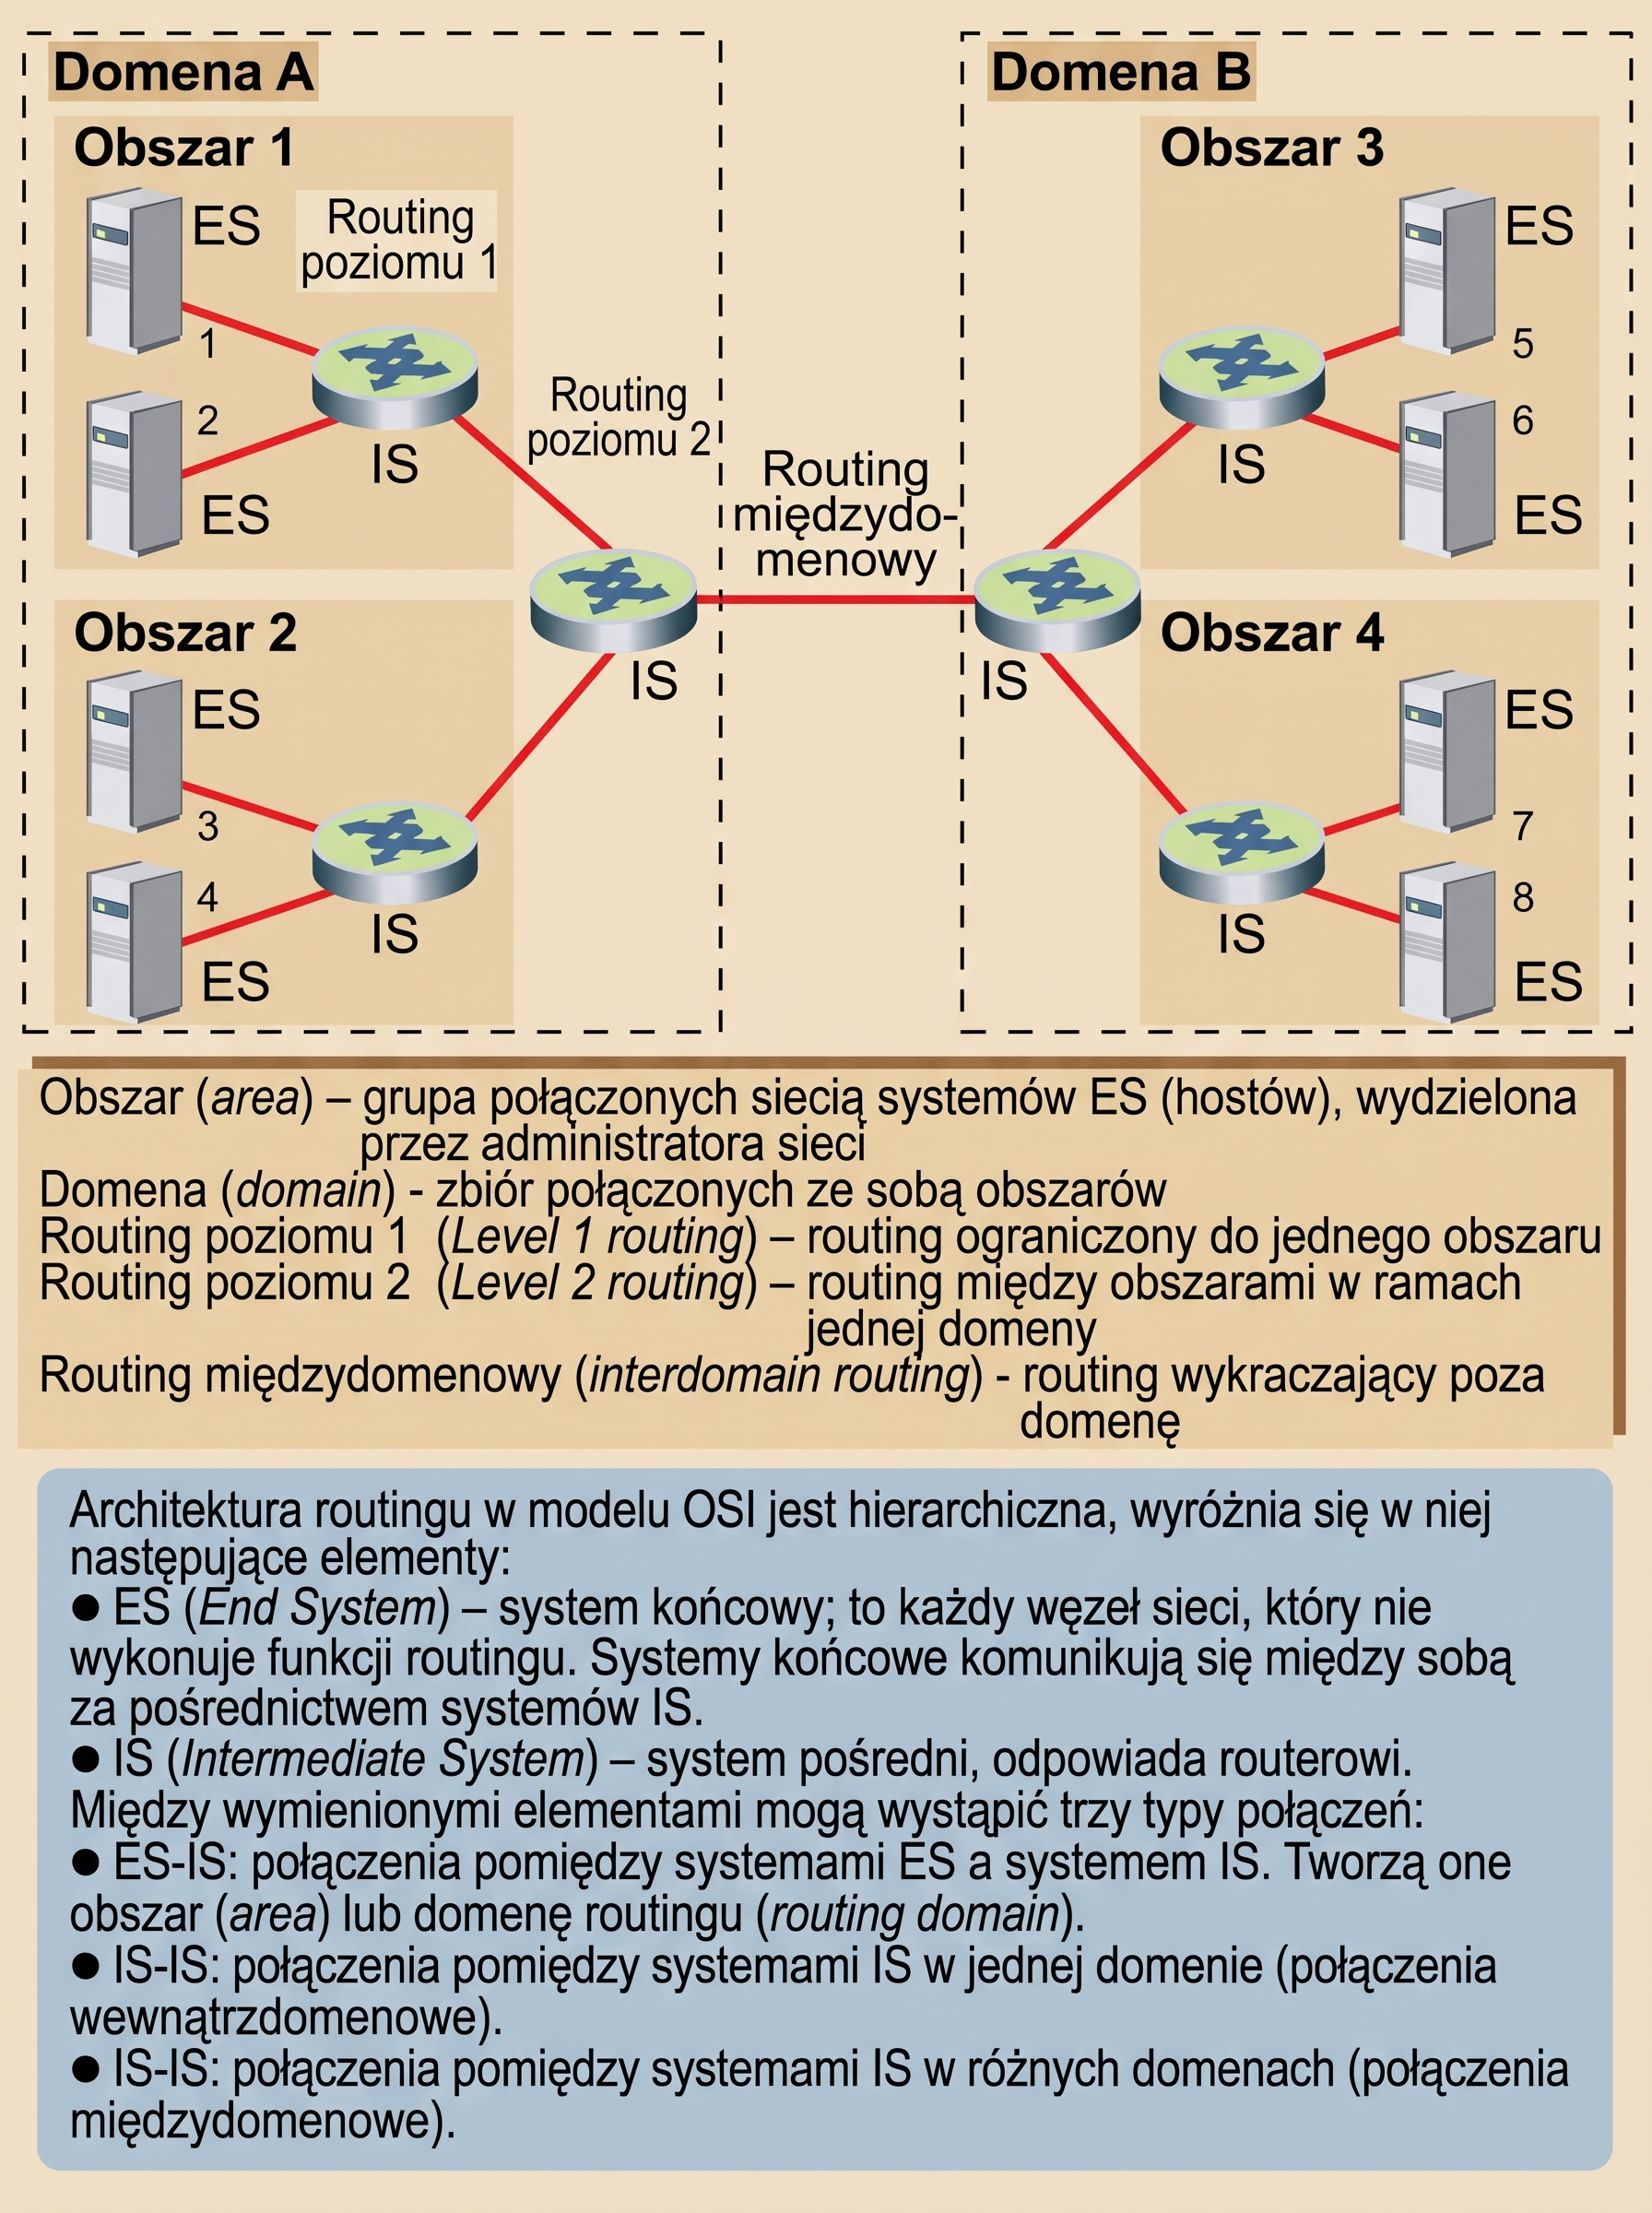
\includegraphics[width=0.8\textwidth]{osi.png}
    \caption{Schemat OSI}
    \label{fig:schemat_osi}
\end{figure}

\subsection{Przegląd wybranych protokołów routingu}
\begin{itemize}
    \item \textbf{RIP (Routing Information Protocol):} protokół typu Distance Vector wykorzystujący jako metrykę liczbę skoków (maksymalnie 15). Pakiety aktualizacji przesyłane są w trybie rozgłoszeniowym z wykorzystaniem protokołu UDP na port 250. Jest stosowany w mniejszych sieciach jako wewnętrzny protokół trasowania IGP (Interior Gateway Protocol), czyli obsługuje routing wewnątrz pojedynczego systemu autonomicznego (w przeciwieństwie do protokołów zewnętrznych EGP, które odpowiadają za routing pomiędzy różnymi systemami autonomicznymi).
    \item \textbf{IGRP (Interior Gateway Routing Protocol):} Ulepszenie RIP z własnym protokołem warstwy transportu: obsługuje do 255 skoków, uwzględnia złożoną metrykę (przepustowość, opóźnienie, obciążenie) oraz oferuje szybszą zbieżność dzięki aktualizacjom \textit{flash}.
    \item \textbf{OSPF (Open Shortest Path First):} otwarty protokół typu \textit{Link State}. Routery OSPF przesyłają ogłoszenia wewnątrz obszaru hierarchicznego i budują pełną mapę topologii, wykorzystując algorytm Dijkstry (oblicza najkrótszą trasę do każdego węzła). Zapewnia szybką zbieżność oraz wspiera uwierzytelnianie i podział na obszary.
\end{itemize}

\subsection{Narzędzia diagnostyki sieciowej}
Do weryfikacji i analizy ścieżek pakietów w ramach laboratoryjnej części ćwiczenia wykorzystamy standardowe narzędzia systemowe:
\begin{itemize}
    \item \textbf{ping:} narzędzie diagnostyczne sieci TCP/IP. Umożliwia weryfikację dostępności hosta, pomiar opóźnień oraz oszacowanie poziomu straty pakietów.
    \item \textbf{traceroute:} aplikacja służąca do badania dokładnej trasy pakietu od źródła do celu. Dzięki niej możliwe jest wyznaczenie  opóźnień na każdym skoku.
\end{itemize}





\end{document}